\section{Results}\label{sec:results}
% Primary: Thomas & all

\subsection{LANL APEX Simulation Workflows on Celio}

We consider the workload from LANL found in the APEX Workflows
report~\cite{apex} that consists of four simulation applications
classes: EAP, LAP, Silverton and VPIC. The main characteristics of
these classes are reported in Table~\ref{table:lanl}. We simulate the
behavior of these applications over the Celio Platform. \todo{Describe
  Celio here}

\begin{table}
\begin{tabular}{|l|c|c|c|c|}
\hline
 Workflow & EAP & LAP & Silverton & VPIC \\\hline
Workload percentage & 66 & 5.5 & 16.5 & 12 \\\hline
Work time (h) & 262.4 & 64 & 128 & 157.2 \\\hline
Number of cores & 16384 & 4096 & 32768 & 30000 \\\hline
Initial Input (\% of memory) &  3 & 5 & 70 & 10 \\\hline
Final Output (\% of memory) & 105 & 220 & 43 & 270 \\\hline
Checkpoint Size (\% of memory) & 160 & 185 & 350 & 85 \\\hline
\end{tabular}
\caption{LANL Workflow Workload from the APEX Workflows report\label{table:lanl}}
\end{table}

Enough applications are randomly chosen to ensure that the workload
percentage of each class is met within 1\% of its goal, and to gather
a simulated time of at least 2 months (62 days). To serve as the
baseline of comparison, we simulate the execution of each list of
applications without introducing checkpoints, faults, or
interference. In this simulation, we select a segment of the execution
that is 60 days long (to exclude the beginning and end of the
simulation that present uncharacteristic behaviors), and compute 
the resource used by the applications during that time. Since we
consider efficiency from a platform perspective and each application
has a different resource usage, we use the following metric to measure
resource usage: the sum of time each node spends doing a specific
operation. Application usage sums the time spent doing I/O or
computation that was not wasted by a restart due to a failure.

For each checkpointing and I/O scheduling technique presented in
Section~\ref{sec:algorithm}, we then compute the resource waste, as
the sum of application computation or I/O that was wasted due to
failures, and of time checkpointing. We represent below the
performance of each technique by computing the waste ratio, i.e. the
waste resource over a segment of 60 hours divided by the application
usage resource over that same segment for the baseline
simulation. Each simulation is conducted 2,000 times, and the
candelstick extremes represent the first and last decile of the
measures, while the boxes represent the second and third quartile, and
the point in the middle the mean value.

\begin{figure}
  \begin{center}
    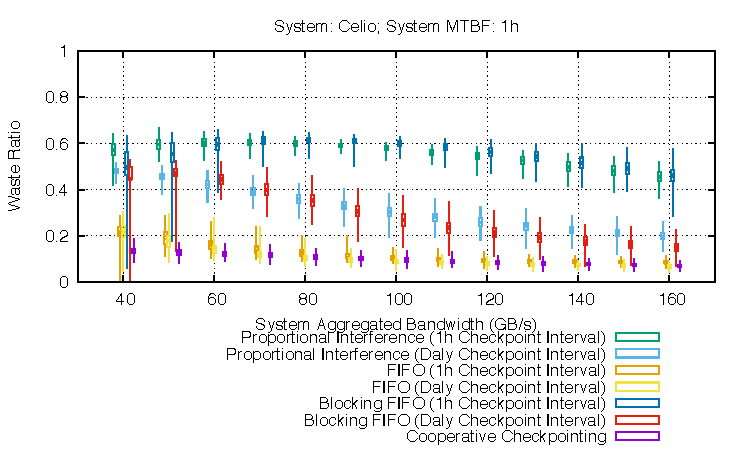
\includegraphics[width=\linewidth]{sim/figures/synthetic-01hMTBF-waste-celio.pdf}
  \end{center}
  \caption{Waste ratio as a function of the system bandwidth for the
    seven I/O and Checkpointing scheduling strategies, and the Celio
    workload \label{fig:celio-1hmtbf}}
\end{figure}

First, we explore the performance of each approach under heavy risks
of failures. Figure~\ref{fig:celio-1hmtbf} represents the waste ratio
on Celio, assuming the MTBF of the system was 1h. We vary the
filesystem bandwidth from 40 GB/s to 160GB/s in order to evaluate the
impact of this parameter. We observe 3 classes of behavior: \propfixed
and \bfifofixed exhibit a waste ratio that decrease as the bandwidth
increases, but remains above 40\% even with a high available
bandwidth; \fifodaly, \fifofixed, and \cooperative quickly decrese at
only 20\% of waste or less, and reach the theoretical model
performance; and \propdaly and \bfifodaly start at the same level of
efficiency as \propfixed and \bfifofixed, and reach the 20\% of waste
as the bandwidth increases.

This figure shows that with a high frequency of failures, providing
each application with the appropriate checkpoint interval is central
to relieve the filesystem from unecessary (or even detrimental)
checkpoints, but this is not the sole criteria that should be taken
into account. The two strategies that remain with a high waste despite
a high bandwidth rely on a fixed 1h interval. As the figure
illustrates, simply relying on the Daly checkpointing period is not
sufficient to reach the best performance under constrained bandwidth:
at 60GB/s for the filesystem, \propdaly and \bfifodaly experience
twice the waste of the other strategies relying on the same value for
the checkpointing period. All strategies that decouple the execution
of the application from the filesystem availability (\fifodaly,
\fifofixed, \cooperative) exhibit much better performance despite low
bandwidth. 

Notably, \cooperative remains the most efficient technique under all
conditions, and reaches the theoretical performance given by
Equation~\ref{eq.totalwaste} in the case of a stead state
analysis. This illustrates the efficiency of the proposed heuristic
(Equations~\ref{eq.heuristicpart1} and~\ref{eq.heuristicpart2}) to
schedule checkpoints and I/O in a way that avoids interferences,
allowing the system to behave as if no interference was experienced,
in most cases. The high variation shows that a minority of the runs
experienced a significantly higher waste.

\begin{figure}
  \begin{center}
    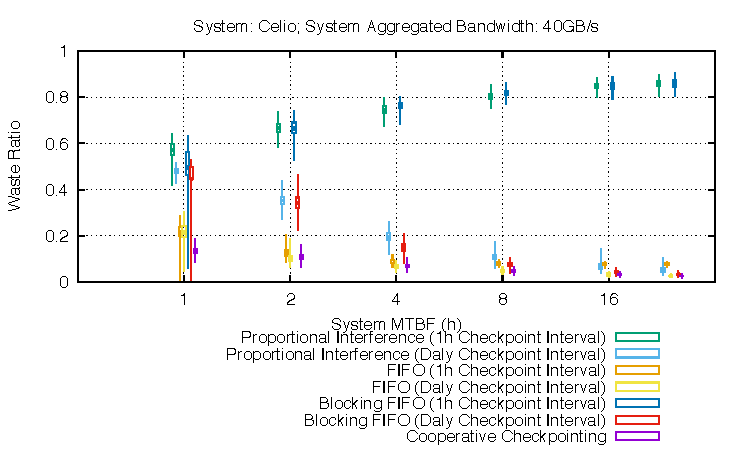
\includegraphics[width=\linewidth]{sim/figures/synthetic-040gbs-waste-celio.pdf}
  \end{center}
  \caption{Waste ratio as a function of the system MTBF for the
    seven I/O and Checkpointing scheduling strategies, and the Celio
    workload \label{fig:celio-40gbs}}
\end{figure}

Second, we explore the performance of each approach under low
bandwidth (and thus high risk of
interference). Figure~\ref{fig:celio-40gbs} represents the waste ratio
on Celio, assuming the aggregated filesystem bandwidth of the system
was 40GB/s. We vary the system MTBF from 1h (2 years of node MTBF) to
24h (48 years of node MTBF) in order to evaluate the impact of this
parameter. Similarly to Figure~\ref{fig:celio-1hmtbf}, we observe 3
classes of behavior: \propfixed and \bfifofixed exhibit a waste ratio
that remains constant around 80\% for all values of the MTBF. These
appraoch are critically dependent on the filesystem bandwidth, and a
lower frequency of failures does not significantly improve their
performance. The I/O subsystem is saturated, and the applications
spends most of their time waiting for it. \fifodaly, \fifofixed, and
\cooperative quickly fall at only 20\% of waste or less, and reach
the theoretical model performance; and \propdaly and \bfifodaly start
at the same level of efficiency as \propfixed and \bfifofixed, and
reach the 20\% of waste as the bandwidth increases.

For all the strategies that integrate the Daly checkpointing period
optimization, increasing the MTBF reduces the amount of I/O required
and thus enables to manage a constrained bandwidth easily. All
strategies that schedule the bandwidth are succesful at increasing the
efficiency to values very close to the theoretical model. More
suprisingly, the simple FIFO scheduling of checkpoints with fixed
chekpoint interval (\bfifofixed) is capable of reaching a performance
comparable to the one of the strategies that reduce the number of
checkpoints. This is due to the significant reduction in interference
due to the reduction of number of restarts with an MTBF of 8h. As soon
as the number of restarting applications decreases, the filesystem
sollicitation decreases sufficiently to avoid long delays in non blocking
approaches, as is illustrated by the performance of \fifofixed at 2h
of MTBF.

\subsection{Prospective Systems}

